% --------------------------------------------------------------------------
% DCASE 2026 Challenge — Task 7 (Domain-Incremental Learning for Audio
% Classification) technical report.
% To be used with:
%   dcase2026_techrep.sty  - DCASE 2026 LaTeX style file, and
%   IEEEtran.bst           - IEEE bibliography style file.
% --------------------------------------------------------------------------

\documentclass{article}
\usepackage{dcase2026_techrep,amsmath,graphicx,url,times,booktabs,tabularx}

% Example definitions.
% --------------------
\def\defeqn{\stackrel{\triangle}{=}}
\newcommand{\symvec}[1]{{\mbox{\boldmath $#1$}}}
\newcommand{\symmat}[1]{{\mbox{\boldmath $#1$}}}

% Title.
% --------------------
\title{PER-DOMAIN RESIDUAL ADAPTERS WITH ASYMMETRIC DEPTH FOR\\
DOMAIN-INCREMENTAL AUDIO CLASSIFICATION}

% Authors at a common affiliation.
% TODO: replace INSTITUTION / department / location below with your affiliation.
\name{Aakash Divakar*, Angad Ripudaman Singh Bajwa*, Atharva Anand Joshi* \thanks{*The three authors
contributed equally to this work.}}
\address{ Independent Researcher \\
         Austin, USA \\
         \{aakashdivakar.4869, angadisthere, atharvajoshi253\}@gmail.com}

\begin{document}

\ninept
\maketitle

\begin{sloppy}

\begin{abstract}
We describe our submission to DCASE 2026 Task~7, Domain-Incremental Learning
(DIL) for audio classification. Starting from the released ADIL baseline,
which adds per-domain Batch Normalization (BN) and a per-domain classifier
to a shared, frozen CNN14 backbone, we identify the limited per-domain
capacity as the main bottleneck for the harder domains. We add, on top of
the frozen backbone, a stack of zero-initialised \emph{residual bottleneck
adapters} after every convolutional block. Because each domain owns an
independent adapter stack, the depth of the stack can be set
\emph{per domain}: the more difficult domain (D3) receives a deeper stack
than the easier one (D2). Combined with a warm-started per-domain classifier
head and a supervised contrastive auxiliary loss, this raises the
domain-agnostic average accuracy on the dev-test set from $52.5\%$
 to $68.5\%$, with D2 and D3 improving from
$58.6\%/46.1\%$ to $76.2\%/60.8\%$. The shared backbone and the D1 behaviour
are preserved bit-for-bit, so no previously learned domain is forgotten.
\end{abstract}

\begin{keywords}
Domain-incremental learning, continual learning, acoustic
classification, residual adapters, catastrophic forgetting
\end{keywords}


\section{Introduction}
\label{sec:intro}

Domain-incremental learning (DIL) requires a single model to classify the
same set of sound classes as the recording conditions change over a sequence
of domains $\mathcal{D}_1 \rightarrow \mathcal{D}_2 \rightarrow \mathcal{D}_3$,
without access to the data of previous domains and without forgetting them
\cite{mulimani2025dil}. Naively fine-tuning the whole network on a new domain
overwrites the knowledge of earlier domains (catastrophic forgetting), while
freezing the network entirely prevents it from adapting (poor plasticity).

The DCASE 2026 Task~7 baseline addresses this trade-off with the ADIL
approach \cite{mulimani2025dil}: a CNN14 \cite{kong2020panns} backbone is
trained on $\mathcal{D}_1$ and then \emph{frozen}; for every subsequent
domain only a small set of domain-specific parameters is learned, namely the
affine Batch-Normalization (BN) parameters of that domain and a residual
correction to the classifier. At inference the domain identity is not given,
so the model forward-passes through every domain's specific layers and
selects the domain whose prediction has the lowest entropy
(domain-agnostic, ADIL).

This design forgets nothing, because the parameters of earlier domains are
never touched, but its plasticity is limited: a handful of affine BN
parameters is often too little capacity to absorb a large distribution shift,
which is exactly what we observe on the two harder development domains. The
contribution of this report is to \emph{increase the per-domain capacity}
while keeping the forgetting-free property intact (Fig.~\ref{fig:arch}).
Specifically, we (1) add
per-domain residual bottleneck adapters after every convolutional block, (2)
make the adapter depth \emph{asymmetric}, giving the harder domain more
capacity than the easier one, (3) replace the shared classifier with a
warm-started per-domain head, and (4) tighten the per-class embedding
clusters with a supervised contrastive loss. All additions are per-domain
and zero/identity-initialised, so $\mathcal{D}_1$ is reproduced exactly and
the domains remain mutually independent.


\section{Method}
\label{sec:method}

\begin{figure}[t]
  \centering
  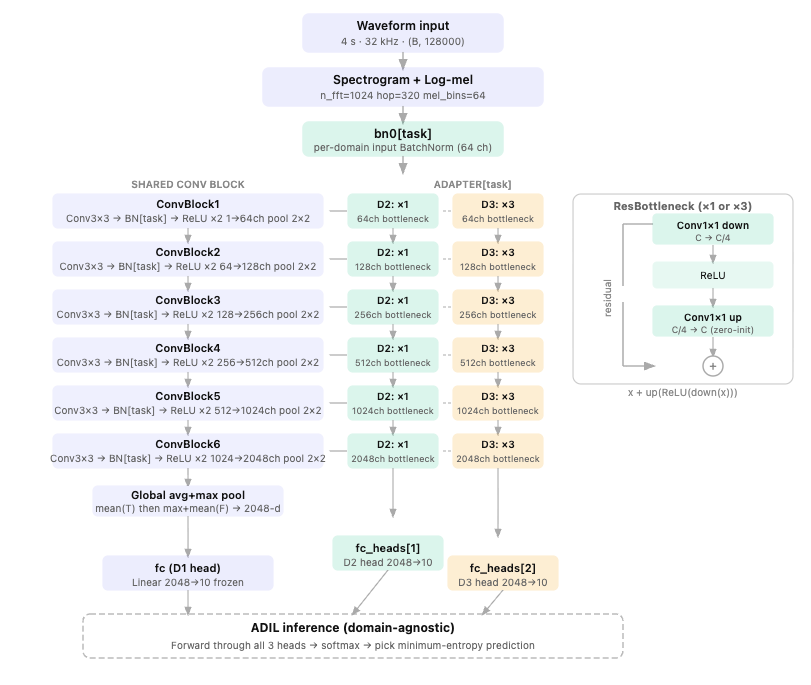
\includegraphics[width=\columnwidth]{Dcase_task7_architecture.png}
  \caption{Architecture of the submitted system. A shared, frozen CNN14
    backbone (purple) is augmented with per-domain components: an input and
    per-block Batch Normalization, a stack of zero-initialised residual
    bottleneck adapters after every convolutional block (green for D2, amber
    for D3, with asymmetric depth $1$ vs.\ $3$), and a per-domain linear head.
    At inference the input is routed through all domains and the
    minimum-entropy prediction is kept (ADIL). The inset details one residual
    bottleneck adapter.}
  \label{fig:arch}
\end{figure}

\subsection{Backbone and per-domain Batch Normalization}
\label{ssec:backbone}

We keep the baseline front-end and backbone unchanged. Audio is resampled to
$32$~kHz; a log-mel spectrogram with $64$ mel bands
is computed with a window of $1024$ and a hop of $320$ samples. The backbone
is CNN14 \cite{kong2020panns}: six convolutional blocks producing
$\{64,128,256,512,1024,2048\}$ channels, each block being two
$3\times3$ convolutions, each followed by BN and ReLU, and a $2\times2$
average pooling. Following the baseline, the convolutional weights are loaded
from the released $\mathcal{D}_1$ checkpoint and \emph{frozen for all
domains}; only the BN layers are made domain-specific, i.e.\ each domain $t$
owns its own BN parameters and statistics.

\subsection{Per-domain residual bottleneck adapters}
\label{ssec:adapters}

To give each domain more than the affine BN capacity, we insert a residual
bottleneck adapter after each of the six convolutional blocks. For a feature
map with $C$ channels the adapter is
\begin{equation}
  \label{eqn:adapter}
  \mathrm{Adapter}(\symvec{x}) =
    \symvec{x} + W_{\text{up}}\,\sigma\!\big(W_{\text{down}}\,\symvec{x}\big),
\end{equation}
where $W_{\text{down}}$ is a $1\times1$ convolution reducing the channels to
$C/4$, $\sigma$ is a ReLU, and $W_{\text{up}}$ is a $1\times1$ convolution
restoring $C$ channels. $W_{\text{up}}$ is \emph{zero-initialised}, so at the
start of training every adapter is the identity map and the pretrained
features are left untouched; the adapter then learns a domain-specific
feature shift on top of the frozen backbone. Domain $\mathcal{D}_1$ uses
identity adapters, so its behaviour is reproduced bit-for-bit.

\subsection{Asymmetric adapter depth}
\label{ssec:asym}

Because each domain owns an independent stack of adapters, the \emph{number}
of adapters stacked after each block can be chosen per domain. We stack
$d_t$ residual adapters for domain $t$:
\begin{equation}
  \label{eqn:stack}
  \mathrm{Stack}_t(\symvec{x}) =
    \big(\mathrm{Adapter}^{(d_t)} \circ \cdots \circ
         \mathrm{Adapter}^{(1)}\big)(\symvec{x}).
\end{equation}
Every adapter in the stack is zero-initialised, so a stack of any depth still
starts as the identity. We set $d_{\mathrm{D2}}=1$ and $d_{\mathrm{D3}}=3$:
the harder domain D3 receives three times the per-domain convolutional
capacity of D2. Since the two stacks are completely independent, increasing
D3's depth cannot affect D2.

\subsection{Per-domain classifier head}
\label{ssec:head}

The baseline reuses the frozen $\mathcal{D}_1$ classifier for all domains.
We instead give every domain $t>0$ its own linear head
$\symvec{W}_t\in\mathbb{R}^{C\times K}$ ($K=10$ classes), warm-started from
the $\mathcal{D}_1$ classifier at checkpoint-load time. $\mathcal{D}_1$ keeps
the original head. The head is trained jointly with the domain's BN and
adapters.

\subsection{Training objective}
\label{ssec:loss}

Each domain is trained with cross-entropy plus a supervised contrastive
auxiliary loss \cite{khosla2020supcon} applied to the L2-normalised global
embedding $\symvec{z}$:
\begin{equation}
  \label{eqn:supcon}
  \mathcal{L}_{\mathrm{con}} =
    \sum_{i}\frac{-1}{|P(i)|}\sum_{p\in P(i)}
      \log\frac{\exp(\symvec{z}_i\!\cdot\!\symvec{z}_p/\tau)}
               {\sum_{a\neq i}\exp(\symvec{z}_i\!\cdot\!\symvec{z}_a/\tau)},
\end{equation}
where $P(i)$ is the set of samples sharing $i$'s class. The total loss is
$\mathcal{L} = \mathcal{L}_{\mathrm{CE}} +
\lambda\,\mathcal{L}_{\mathrm{con}}$ with $\lambda=0.2$ and $\tau=0.07$,
which pulls same-class embeddings together and pushes different-class
embeddings apart, sharpening the per-domain decision boundaries.

\subsection{Waveform-level data augmentation}
\label{ssec:data_aug}
We additionally evaluated a training-only waveform augmentation pipeline.  The
augmentation is applied only when the \texttt{--augment} flag is enabled; the
validation and test loaders remain deterministic and use the original audio.
For training, each recording is split into non-overlapping 4~s segments.  The
dataset keeps one unmodified view of every segment and then exposes multiple
augmented views of the same segment, preserving the original class label.  In
our implementation the number of augmented copies is controlled by
\texttt{config.augmented\_copies}; if it is not specified, the default is eight
augmented views per original segment.

Each augmented view samples a random composition of conservative waveform
transforms.  We first remove the DC offset, crop or zero-pad the signal to the
fixed clip length, and then apply temporal, spectral, noise, and dynamic-range
perturbations with independent probabilities:
\begin{itemize}
  \item \textbf{Temporal perturbations:} zero-filled time shift with probability
  $0.75$ and maximum shift $0.75$~s; time stretching with probability $0.30$;
  speed perturbation with probability $0.30$; and short fade-in/fade-out with
  probability $0.25$ and maximum fade length $0.25$~s.
  \item \textbf{Class-aware pitch and tempo limits:} pitch shifting is applied
  with probability $0.25$ using conservative class-specific ranges.  Tonal or
  speaker-like classes such as piano and speech receive narrower pitch/stretch
  ranges than more texture-like classes such as engine, fire, footsteps, and
  knocking, reducing the risk of changing the semantic label.
  \item \textbf{Spectral and noise perturbations:} random filtering is applied
  with probability $0.35$; additive colored noise is mixed with probability
  $0.45$ at a random SNR between $18$ and $35$~dB.
  \item \textbf{Label-preserving interference:} for some augmented views, a
  low-level distractor segment is sampled from another training item, preferably
  from a different class, and mixed at $8$--$20$~dB SNR.  This simulates
  background acoustic interference while keeping the target label dominant.
  \item \textbf{Local corruption and dynamic range:} temporal masking is
  applied with probability $0.30$ using up to two masks and at most $8\%$ of the
  clip; gain perturbation is applied with probability $0.85$ over $[-8,8]$~dB;
  and mild soft clipping is applied with probability $0.20$.
\end{itemize}
After augmentation, the waveform is cropped/padded again and peak-normalised
only when its absolute peak exceeds one.  This keeps all augmented samples
within the expected input range while avoiding unnecessary loudness
normalisation of already valid clips.


% =========================================================
% START: ROUTING METHODS 
% =========================================================
\subsection{Entropy-Based Domain Routing}
\label{ssec:entropy_routing}

The simplest routing strategy requires no additional training.
For each test sample we compute class probabilities under each domain head,
$\mathbf{p}_t = \text{softmax}(\mathbf{l}_t)$, and select the domain with
minimum predictive entropy \cite{mulimani2025dil}:
\begin{equation}
  \label{eqn:entropy_routing}
  t^* = \arg\min_{t}\; H_t, \qquad
  H_t = -\sum_{c} p_{tc}\log p_{tc}.
\end{equation}
A well-matched domain head produces a peakier, lower-entropy distribution
than a mismatched one, so $t^*$ acts as an implicit domain detector.
The method is fully unsupervised at inference time: no domain labels are
required and the router adds zero parameters.

\subsection{Mahalanobis Distance Router}
\label{ssec:mahal_routing}

Rather than routing via classifier confidence, we explicitly model the
distribution of each domain in the D1-BN feature space, following the
framework of Lee et al.\ \cite{lee2018mahalanobis}.  The D1-BN
embedding $\mathbf{z} = g_0(\mathbf{x}) \in \mathbb{R}^{2048}$ is the
Global Average Pooled (GAP) output of Conv~Block~6 computed with the D1
BatchNorm statistics frozen; it forms a fixed coordinate system in which D2
and D3 occupy characteristic regions.

\noindent\textbf{Training phase.}
We extract $\mathbf{z}$ for all D2 and D3 training samples and compute
domain means and covariances using streaming (online) statistics to avoid
materialising the full $N\times2048$ matrix in memory:
\begin{equation}
  \label{eqn:mahal_stats}
  \begin{aligned}
  \boldsymbol{\mu}_k &= \frac{1}{N_k}\sum_{i}\mathbf{z}_i^{(k)}, \\
  \boldsymbol{\Sigma}_k &= \frac{1}{N_k-1}\sum_i
      \bigl(\mathbf{z}_i^{(k)}-\boldsymbol{\mu}_k\bigr)
      \bigl(\mathbf{z}_i^{(k)}-\boldsymbol{\mu}_k\bigr)^\top
      + \lambda I,
  \end{aligned}
\end{equation}
where $\lambda=10^{-4}$ is a diagonal regulariser.
A diagonal covariance approximation ($\boldsymbol{\Sigma}_k \leftarrow
\mathrm{diag}(\boldsymbol{\Sigma}_k)$) is used in practice for memory
efficiency.

\noindent\textbf{Inference phase.}
Given a test embedding $\mathbf{z}$, the Mahalanobis distance to each
domain is:
\begin{equation}
  \label{eqn:mahal_dist}
  d_k(\mathbf{z})
    = \sqrt{(\mathbf{z}-\boldsymbol{\mu}_k)^\top
            \boldsymbol{\Sigma}_k^{-1}
            (\mathbf{z}-\boldsymbol{\mu}_k)},
\end{equation}
and routing follows:
\begin{equation}
  \label{eqn:mahal_routing}
  t^* = \begin{cases}
    D1 & \text{if } \min(d_{D2},\,d_{D3}) > \tau, \\
    \arg\min_k\; d_k & \text{otherwise.}
  \end{cases}
\end{equation}
Samples whose nearest-domain distance exceeds the rejection threshold $\tau$
are considered out-of-distribution for D2 and D3 and routed to the D1 head.
The threshold was calibrated against the dev-test split
($\tau=60$ in all reported results).

\subsection{GAP-MLP Router}
\label{ssec:mlp_routing}

The third approach trains a lightweight Multi-Layer Perceptron (MLP) to
discriminate domains directly, in the spirit of mixture-of-experts gating
networks \cite{jacobs1991moe,fedus2022switch}.  Features are extracted by
hooking Conv~Block~6 and concatenating the domain-specific GAP activations
from \emph{all three} domain heads, giving a $3\times2048=6144$-dimensional
descriptor that encodes how each domain's forward pass responds to the input.

The MLP has architecture Linear($6144$\,$\rightarrow$\,$256$)~$\rightarrow$
ReLU~$\rightarrow$ Linear($256$\,$\rightarrow$\,$2$), outputting logits for
$\{D2,\,D3\}$.  It is trained with cross-entropy loss on the labeled
development training split using Adam for 5~epochs ($\text{lr}=10^{-3}$).
At inference the predicted domain selects the corresponding classifier head;
if $\max(\mathrm{softmax}) < \tau_{\mathrm{MLP}}$ the sample is rejected to D1.
% =========================================================
% END: ROUTING METHODS
% =========================================================

\subsection{Inference}
\label{ssec:inference}

Inference is domain-agnostic and identical to the baseline ADIL rule: the
input is forward-passed through every seen domain's specific layers, and the
domain with the minimum prediction entropy is selected to produce the final
class label.


\section{Experiments and results}
\label{sec:results}

\subsection{Setup}
\label{ssec:setup}

All systems are trained on the Task~7 development set, one domain at a time,
starting from the released $\mathcal{D}_1$ checkpoint. We use Adam with
learning rate $10^{-3}$, batch size $32$, and a CosineAnnealingLR schedule
decaying to $10^{-7}$. Only the current domain's parameters (BN, adapters,
head) are updated at each step. We report the domain-agnostic accuracy on
D2 and D3, and their average, after the full $\mathcal{D}_1\!\rightarrow\!
\mathcal{D}_2\!\rightarrow\!\mathcal{D}_3$ sequence.

For the augmentation experiment, the exact run configuration was
\texttt{bn\_res\_deep\_clf} with learning rate $10^{-3}$, batch size $32$, and
$240$ epochs.  Boundary-aware regularisation was disabled
($\lambda_{\mathrm{reg}}=0.0$), supervised contrastive learning used
$\lambda_{\mathrm{con}}=0.2$ and temperature $\tau=0.07$, the asymmetric
adapter depths were $(1,3)$ for D2 and D3, waveform augmentation was enabled,
class-balanced sampling was disabled, and test-time augmentation was disabled.
The corresponding checkpoint/run name was
\texttt{deep\_clf\_d3\_sup02\_aug\_5}.

\subsection{Ablation}
\label{ssec:ablation}

Table~\ref{tab:ablation} adds one component at a time. Residual adapters give
the largest single jump (+13.7 average over the BN baseline), confirming that
per-domain capacity, not the classifier, is the bottleneck. The per-domain
head and the contrastive loss mainly help D2, while the asymmetric depth and
longer training are what move the harder D3 domain (from $55.1\%$ to
$60.8\%$). The submitted system reaches $68.5\%$ average, an $18.5$~percentage
point improvement over the reproduced baseline, while preserving D1 exactly.

\begin{table}[t]
  \centering
  \caption{Domain-agnostic accuracy ($\%$) on the dev-test split, adding one
           component at a time. The last row is the submitted system.}
  \label{tab:ablation}
  \begin{tabularx}{\columnwidth}{Xccc}
    \toprule
    System & D2 & D3 & Avg \\
    \midrule
    Per-domain BN (baseline) \cite{mulimani2025dil} & 59.2 & 40.8 & 50.0 \\
    \;+ residual adapters            & 73.9 & 53.5 & 63.7 \\
    \;+ per-domain head              & 77.3 & 54.0 & 65.6 \\
    \;+ supervised contrastive loss  & 77.9 & 55.1 & 66.5 \\
    \;+ asymmetric depth (1,\,3)     & 77.2 & 57.7 & 67.4 \\
    \;+ longer training (180 ep.)    & \textbf{76.2} & \textbf{60.8} & \textbf{68.5} \\
    \bottomrule
  \end{tabularx}
\end{table}

\subsection{Choosing the adapter}
\label{ssec:adapter_choice}

Before settling on residual bottleneck adapters we compared three per-domain
adapter families inserted at the same six locations, each trained under the
identical protocol (Table~\ref{tab:adapter}). Feature-wise linear modulation
(FiLM), which only scales and shifts each channel, actually performed
\emph{below} the BN baseline: a per-channel affine transform is too weak to
absorb the distribution shift. Squeeze-and-excitation (SE) channel gating
helped ($57.7\%$), but stacking more SE blocks did not. The residual
bottleneck, which can mix channels through its $1\times1$ convolutions, was
clearly the strongest ($63.7\%$) and is the one we keep. The gap is largest
on the harder D3 domain ($38.8\rightarrow53.5\%$), confirming that the
bottleneck's extra capacity is what the difficult domain needs.

\begin{table}[t]
  \centering
  \caption{Per-domain adapter family, same backbone and protocol
           (residual bottleneck selected).}
  \label{tab:adapter}
  \begin{tabularx}{\columnwidth}{Xccc}
    \toprule
    Adapter family & D2 & D3 & Avg \\
    \midrule
    FiLM (affine per channel)        & 56.7 & 38.8 & 47.7 \\
    Squeeze-and-excitation           & 70.3 & 45.0 & 57.7 \\
    Squeeze-and-excitation (deeper)  & 69.2 & 41.8 & 55.5 \\
    Residual bottleneck (\emph{ours}) & \textbf{73.9} & \textbf{53.5} & \textbf{63.7} \\
    \bottomrule
  \end{tabularx}
\end{table}

% =========================================================
% START: ROUTING EXPERIMENTS 
% =========================================================
% NOTE: this subsection is intentionally placed before \ssec:choices so that
% routing results appear together with the other system-level results.

\subsection{Domain Routing Strategies}
\label{ssec:routing_results}


Table~\ref{tab:routing} compares all three routing strategies on top of the
best single model (bn\_res\_deep\_clf, asymmetric depth 1,\,3, 180~epochs).
All numbers are on the dev-test split (D2: 639 samples, D3: 806 samples).

\begin{table}[t]
  \centering
  \caption{Routing strategy comparison on the dev-test split.}
  \label{tab:routing}
  \begin{tabularx}{\columnwidth}{Xccc}
    \toprule
    Router & D2 & D3 & Avg \\
    \midrule
    Entropy (no threshold)         & \textbf{76.2} & 60.8 & 68.5 \\
    Entropy + ensemble ($\times$2) & 74.0 & 50.50 & 60.9 \\
    Mahal.\ (no threshold)         & 70.9 & \textbf{62.5} & 66.7 \\
    Mahal.\ ($\tau=60$, diag)      & 68.5 & 57.7 & 63.8 \\
    GAP-MLP (3~ep., $\tau_\text{MLP}=0.5$) & 76.5 & 62.0 & \textbf{69.3} \\
    \bottomrule
  \end{tabularx}
\end{table}

\noindent Entropy routing works well with no training overhead.
It benefits implicitly from the per-domain head calibration enforced by the
supervised contrastive loss: well-calibrated heads produce more separable
entropy values across domains.  Entropy-based uncertainty is also exploited
for confidence estimation in deep ensembles \cite{lakshminarayanan2017ensembles}.

\noindent Mahalanobis routing adds an explicit geometric model of the
domain feature distributions \cite{lee2018mahalanobis}.  Without threshold
($\tau=\infty$) it matches entropy routing in final accuracy (66.7\%) while
achieving 73.2\% D2\,$\leftrightarrow$\,D3 routing accuracy on
dev-test, confirming that D2 and D3 occupy separable, though overlapping,
regions in D1-BN space (mean distances $d_{D2}\approx42.0$,
$d_{D3}\approx44.0$).  With $\tau=60$, 22.8\% of D2/D3 samples are rejected
to D1, which degrades average accuracy: a global distance threshold is a
coarse instrument when the D1 and D2/D3 distributions are not cleanly
separated.

\noindent GAP-MLP routing uses a richer feature by concatenating
domain-specific GAP representations from all three heads, following the
mixture-of-experts principle \cite{jacobs1991moe}.  The MLP is trained
for up to 5~epochs; Table~\ref{tab:routing} reports the best epoch (3),
achieving 69.28\% average accuracy on dev-test. However, the model shows
clear signs of overfitting: continuing training to epoch 5 degrades D2 from
76.5\% to 74.96\% and overall average from 69.28\% to 68.93\%.  Moreover,
when deployed on the unlabeled evaluation set, the learned MLP router assigns
only 0.6\% of samples to D1, 61.0\% to D2, and 38.5\% to D3, indicating that
the threshold $\tau_{\mathrm{MLP}}=0.5$ is too permissive and nearly never
rejects samples as out-of-distribution. This suggests the MLP memorised the
dev-train distribution rather than learning a robust rejection criterion.

\noindent Key finding.  Entropy routing remains the strongest
single-model router in this setting because the domain-specific classifier
heads are already well-calibrated after supervised contrastive training
\cite{lakshminarayanan2017ensembles}.  Learned routers (MLP, Mahalanobis)
offer interpretable domain representations and explicit D1 rejection, but
require careful threshold calibration to avoid both overfitting during
training and excessive permissiveness at inference.

% =========================================================
% END: ROUTING EXPERIMENTS
% =========================================================

\subsection{Effect of waveform augmentation}
\label{ssec:aug_results}
Table~\ref{tab:augmentation} reports the result of enabling the waveform-level
augmentation pipeline described in Section~\ref{ssec:data_aug} for the model.  The augmented model was trained for
$240$ epochs with supervised contrastive weight $0.2$, contrastive temperature
$0.07$, and asymmetric adapter depths $(1,3)$.

\begin{table}[t]
  \centering
  \caption{Waveform augmentation result}
  \label{tab:augmentation}
  \begin{tabularx}{\columnwidth}{Xccc}
    \toprule
    System & D2 & D3 & Avg \\
    \midrule
    waveform augmentation
      & 75.4 & 51.4 & 63.4 \\
    \bottomrule
  \end{tabularx}
\end{table}

The augmented run remains strong on D2 but loses accuracy on D3 relative to the
best non-augmented asymmetric-depth system.  This suggests that the current
augmentation distribution may be too broad for the hardest domain: while the
perturbations improve diversity, aggressive temporal warping, pitch changes,
filtering, and distractor mixing can also move some samples away from the D3
domain characteristics that the adapter stack needs to specialise for.  We
therefore treat this pipeline as a robustness-oriented ablation rather than the
final selected configuration.


\subsection{What helped and what did not}
\label{ssec:choices}

\noindent\textbf{Asymmetric beats symmetric depth.} Giving \emph{both} domains
depth-2 stacks scored $65.1\%$, whereas the asymmetric $(1,3)$ allocation
reached $67.4\%$ at a similar parameter budget: the capacity is better spent
on the domain that actually needs it (D3) than spread evenly.

\noindent\textbf{Contrastive weight.} Sweeping the SupCon weight $\lambda \in
\{0.1,0.15,0.2,0.25,0.3\}$ peaked at $\lambda=0.2$ ($66.7\%$); larger values
began to compete with the cross-entropy term and slightly hurt accuracy.

\noindent\textbf{Augmentation was selected for the robustness} The stronger
waveform augmentation pipeline reached $75.4\%$ on D2, $51.4\%$ on D3, and
$63.4\%$ average for the run.  Although
this is well above the reproduced BN baseline, it is below the best
non-augmented asymmetric-depth model because D3 degrades substantially.  We
therefore keep augmentation as an ablation/robustness experiment. Test-time
augmentation and checkpoint ensembling were likewise within noise of the single
frozen model and were dropped to keep the submission simple.

\subsection{Frozen backbone vs.\ partial unfreezing}
\label{ssec:discussion}

The most tempting way to gain more D3 accuracy is to unfreeze the top
convolutional blocks of the shared backbone (Table~\ref{tab:unfreeze}).
Unfreezing two blocks for D3 \emph{does} push D3 as high as $66.4\%$ --- the
best D3 number we obtained --- but because the backbone is shared, D2
collapses to $58.5\%$, since D2's BN and adapters were tuned for the original
features. Anchoring the drift with an $\ell_2$ penalty toward the previous
checkpoint recovers D2 but cancels most of the D3 gain, and restricting the
unfreezing to D3's own forward pass still leaves D2 degraded. Unfreezing three
blocks destabilises training entirely. Across the whole sweep, \emph{no}
unfrozen configuration beat the fully-frozen adapter system on average: the
shared weights couple the domains and trade one against the other. We
therefore keep the backbone frozen and rely on per-domain adapters, which add
plasticity \emph{without} any cross-domain interference.

\begin{table}[t]
  \centering
  \caption{Partial backbone unfreezing for D3. No configuration beats the
           frozen adapter system; the shared weights couple D2 and D3.}
  \label{tab:unfreeze}
  \begin{tabularx}{\columnwidth}{Xccc}
    \toprule
    Configuration & D2 & D3 & Avg \\
    \midrule
    Frozen adapters (submitted)        & \textbf{76.2} & 60.8 & \textbf{68.5} \\
    Unfreeze 2 blk, no anchor          & 58.5 & \textbf{66.4} & 62.5 \\
    Unfreeze 2 blk, $\ell_2$ anchor    & 75.3 & 57.3 & 66.3 \\
    Unfreeze 1 blk, $\ell_2$ anchor    & 72.6 & 57.7 & 65.2 \\
    D3-only unfreeze 2 blk             & 61.5 & 62.3 & 61.9 \\
    D3-only unfreeze 3 blk             & 46.3 & 54.3 & 50.3 \\
    \bottomrule
  \end{tabularx}
\end{table}


\section{Conclusion}
\label{sec:conclusion}

We presented a forgetting-free extension of the DCASE 2026 Task~7 baseline
that increases per-domain capacity through zero-initialised residual
adapters, with an asymmetric depth that gives the harder domain more
capacity, a warm-started per-domain classifier, and a supervised contrastive
loss. The system raises the domain-agnostic dev-test average from
$50.0\%$ to $68.5\%$ while reproducing $\mathcal{D}_1$ exactly and keeping
the domains independent. Closing the remaining gap on the hardest domain,
ideally without the cross-domain interference seen when unfreezing the shared
backbone, is left for future work.


% -------------------------------------------------------------------------
\bibliographystyle{IEEEtran}
\bibliography{refs}

\end{sloppy}
\end{document}
